\section{Visualization}
\label{sec:Visualization}

\textit{Paraver} is the \textit{BSC} tool for trace visualization. Trace events are encoded in \textit{Paraver} format (\textit{.prv}) 
by the \textit{Extrae} tool (see previous section). \textit{Paraver} is a powerful tool that allows users to show many 
views of the trace data by means of different configuration files. Users can manually load, edit or create configuration files to
obtain different trace data views. 

In the following subsections we will explain how to load a trace file into \textit{Paraver}, open the task 
events view by means of an already predefined configuration file, and how to 
adjust the view to properly display the data.

For further information about \textit{Paraver} please visit the following site:
\begin{center}
\url{http://www.bsc.es/computer-sciences/performance-tools/paraver}
\end{center}

\subsection{Trace Loading}
The final trace file in \textit{Paraver} format (.\textit{prv}) can be found at the \textit{base log folder} of the application
execution inside the trace folder. The fastest way to open it is calling directly the \textit{Paraver} binary using the trace-file name
as arugment.
\begin{lstlisting}[language=bash]
compss@bsc:~$ wxparaver /home/compss/.COMPSs/hmmerobj.HMMPfam_01/trace/*.prv
\end{lstlisting}
 
\subsection{Configuration File}
In order to open a view with the task events of the application, an already predefined configuration 
file is provided. To open it, just go in the main window to the ``Load Configuration'' option in 
the menu ``File''. The configuration file is under the following path \textit{/opt/COMPSs/Dependencies/paraver/cfgs/tasks.cfg}. 
After accepting the load of the configuration file, another window will appear to show the view. Figures \ref{fig:trace_1} and
\ref{fig:trace_2} show an example of this process.

\begin{figure}[ht!]
  \centering
    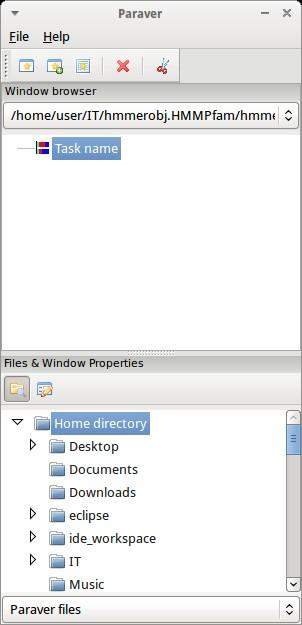
\includegraphics[width=0.45\textwidth]{./Sections/3_Visualization/Figures/1.jpeg}
    \caption{Paraver menu}
    \label{fig:trace_1}
\end{figure}

\begin{figure}[ht!]
  \centering
    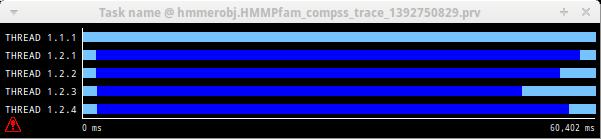
\includegraphics[width=1.0\textwidth]{./Sections/3_Visualization/Figures/2.jpeg}
    \caption{Trace file}
    \label{fig:trace_2}
\end{figure}

\subsection{View Adjustment}
In a \textit{Paraver} view, a red exclamation sign may appear on the bottom-left corner (see last Figure \ref{fig:trace_2} in 
previous section). This means that some little adjustments must be done to view the trace correctly:

\begin{itemize}
 \item Fit window: this will give a better color scale to identify events.
	\begin{itemize}
	    \item Right click on the trace window
	    \item Chose the option Fit Semantic Scale / Fit Both
	\end{itemize}
\end{itemize}

\begin{figure}[ht!]
  \centering
    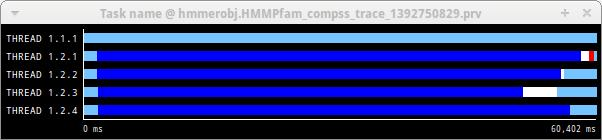
\includegraphics[width=1.0\textwidth]{./Sections/3_Visualization/Figures/3.jpeg}
    \caption{Paraver view adjustment: Fit window}
\end{figure}

\begin{itemize} 
 \item View Event Flags: This will put a flag whenever an event starts/ends.
	\begin{itemize}
	    \item Right click on the trace window
	    \item Chose the option View / Event Flags
	\end{itemize}
\end{itemize}
 
\begin{figure}[ht!]
  \centering
    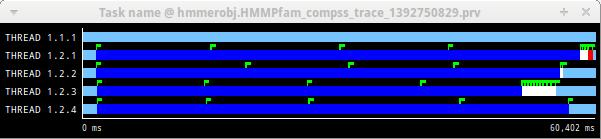
\includegraphics[width=1.0\textwidth]{./Sections/3_Visualization/Figures/4.jpeg}
    \caption{Paraver view adjustment: View Event Flags}
\end{figure}

\begin{itemize}
 \item Show Info Panel: This will show an information panel. In the tab ``Colors'' we can see the legend of the colors shown in the view.
	\begin{itemize}
	    \item Right click on the trace window
	    \item Check the Info Panel option
	    \item Select the Colors tab in the panel
	\end{itemize}
\end{itemize}

\begin{figure}[ht!]
  \centering
    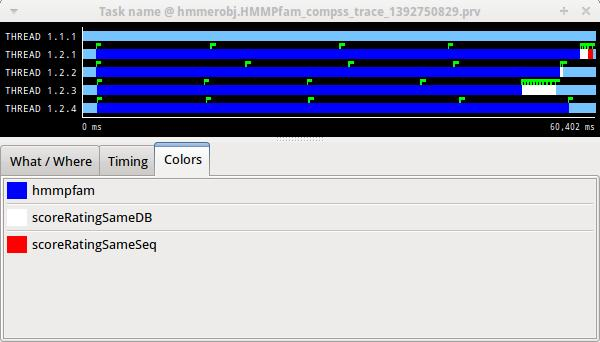
\includegraphics[width=1.0\textwidth]{./Sections/3_Visualization/Figures/5.jpeg}
    \caption{Paraver view adjustment: Show info panel}
\end{figure}

\begin{itemize}
 \item Zoom: In order to understand a trace view better, sometimes it’s a worth thing to zoom into it a little.
	\begin{itemize}
	    \item Select a region in the trace window to see that region in detail
	    \item And repeat the previous step as many times as needed
	    \item The undo-zoom option is in the right click panel
	\end{itemize}
\end{itemize}

\begin{figure}[ht!]
  \centering
    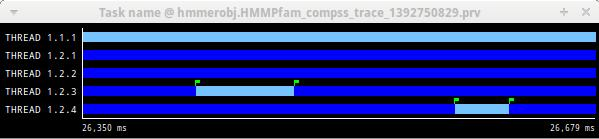
\includegraphics[width=1.0\textwidth]{./Sections/3_Visualization/Figures/6.jpeg}
    \caption{Paraver view adjustment: Zoom configuration}
\end{figure}

\begin{figure}[ht!]
  \centering
    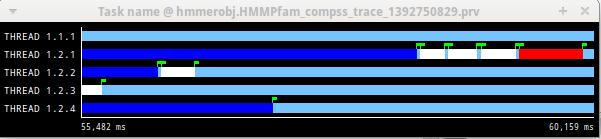
\includegraphics[width=1.0\textwidth]{./Sections/3_Visualization/Figures/6_2.jpeg}
    \caption{Paraver view adjustment: Zoom configuration}
\end{figure}
